%in_memory_file_system

\begin{figure}[t!]
\begin{center}
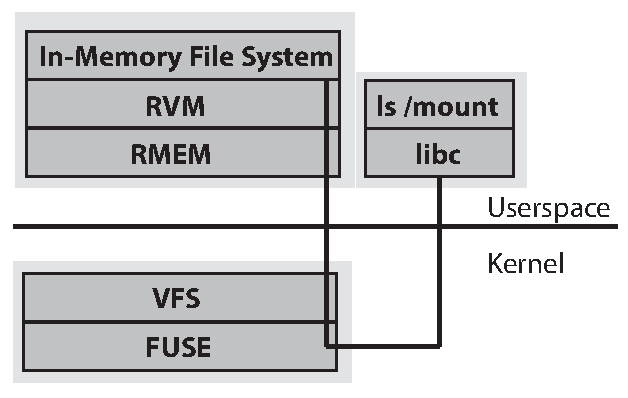
\includegraphics[scale=0.60]{graphs/inmem_fs_design.pdf}
\end{center}
\caption{In-memory file system design when using the RVM framework and FUSE library.}
\label{fig:inmem_fs_design}
\end{figure}

To demonstrate the flexibility and applicability of our framework we have applied our framework to a VFS compliant in-memory file system (see Figure~\ref{fig:inmem_fs_design}). 
Our file system uses main memory as the only storage medium to provide very fast writes and reads. 
To be able to use our framework we have developed the file system using FUSE, a kernel module that allows the creation of user-space file systems.
The decision of running our file system in user-space greatly simplified the development and debugging of both the file system as well as the framework. 
First, because we have no restrictions in the type of system calls we can use we were able to use our framework without major changes to the design and code of RVM.
Secondly, we were able to use tools like GDB or Valgrind to iterate quickly while debugging.



